Items that are cited: \textit{The \LaTeX\ Companion} book \cite{latexcompanion}, The Einstein's journal paper \cite{einstein} and the Dirac's book \cite{dirac} are physics related items. Next, a citation about \textit{The \LaTeX\ Companion} book \cite{latexcompanion} \cite{Koppe}
\cite{Koppe2}


%From the regression analysis, as one could predict, VS units emerged to be correlated with the $Q$ values, in particular FSI units show this correlation very clear.


%\begin{figure}
 %   \centering
 %   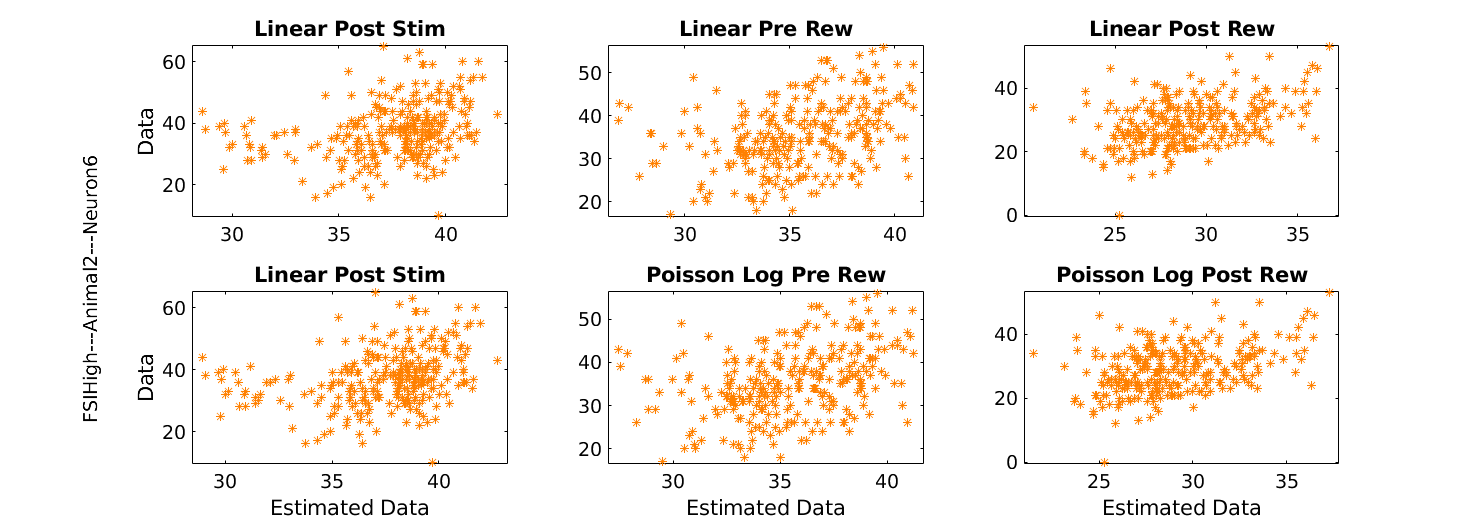
\includegraphics[scale=0.3]{figures/y_yhatAnimal2neu6_FSI.png}
 %   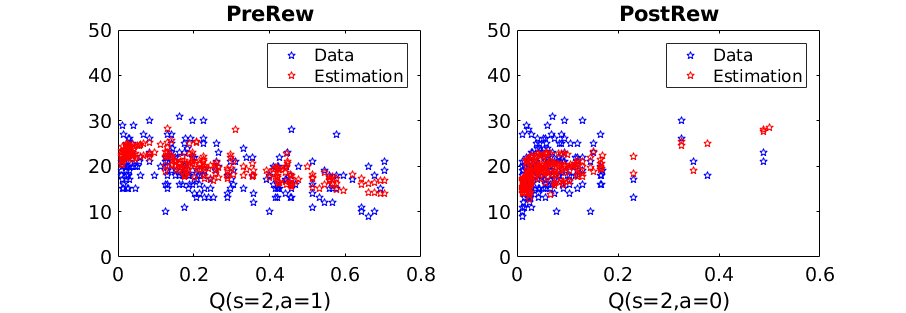
\includegraphics[scale=0.3]{figures/CorrelationExAn1neu6_RightAx.png}
  %  \caption{Caption}
 %   \label{fig:my_label}
%\end{figure}

%We carried out a multiple regression analysis of neuronal and assembly's activity by the four action values of the Q F-L model, $\delta(t)$, $\alpha_L(t)$ and $\alpha_F(t)$. To further test whether the neuronal and assembly activities were correlated with the parameters of subsequent lick movements, or the odor identity, we analyzed the residual components, $\epsilon(t)$, using lick related variables and the odor identity, namely, the mouse's action choice $a(t)$, the lick frequency within the lick-window $l_{in}(t)$, the lick frequency outside the lick-window, before the opening,$l_{out}(t)$ and the odor identity $o(t)$.
%Thus we model the neuronal or assembly activity $y(t)$ during the post-stimulus, pre-reward and post-reward periods in the $t-th$ trial as follows:\\
%\begin{equation}
%\begin{cases}
%y(t)=b_0+\sum\limits_{l}^{L} b_l\cdot M_l+\epsilon(t)\\
%\epsilon(t)=\sum\limits_i^I c_i\cdot N_i
%\end{cases}
%\label{eq:MultiLinRe}
%\end{equation}
%where $y$ are the observations, the neuronal{\color{blue}/assembly's} activity in this case, $M$ is the ($T\times L$) regressor's Matrix of the Q L-F model part, where $T$ is the number of trials and $L$ the number of regressors. $M$ has as columns
%the regressors of the model's part, namely, the vectors $Q_{1,1}$, $Q_{1,0}$, $Q_{2,1}$, $Q_{2,0}$, $\delta$, $\alpha_L$, $\alpha_F$; the set of values $b_m$ are regressor parameters or weights related to the model's regressors. $N$ is the ($T\times I$) regressor matrix of the residual part, where $I$ is the number of regressors of the residual part. N has as columns the regressors $a$, $l_{in}$, $l_{out}$ and $o$, while $c_i$ are the weights of the residual part.
%Linear regression models assume response variables to be normally distributed. Neuronal responses are Poisson distributed (although the normal distribution is in this case a good approximation), {\color{blue} and assemblies show Gamma distribution,} thus considering our data distributions, we built a generalized linear model (GLM), with GLM is possible to generalize the simple linear regression by allowing for response variables that have arbitrary distributions and for an arbitrary function of response variables, the link function, to vary linearly with the predicted values, rather than assuming that the response itself must vary linearly. The mean $\mu$ of distributions depends on the independent variables, or the regressors, $X$, as follows:
%\begin{equation}
%E(Y)=\mu=g^{-1}(X\cdot \beta)
%\label{eq:GLM}
%\end{equation}
%where $g$ is the link function. There is always a well-defined canonical link function which is derived from the exponential of the response's density function. For Poisson observation the canonical link function is the logarithmic. Thus the neuronal activities mean can be expressed by the following:
%\begin{equation}
%\begin{cases}
%\log(\mu)=b_0+\sum\limits_l^L b_l\cdot %M_l+\epsilon(t)\\
%\epsilon(t)=\sum\limits_i^I c_i\cdot N_i 
%\end{cases}
%\label{eq:PoisLinRe}
%\end{equation}